\documentclass{article}
\usepackage[utf8]{inputenc}
\usepackage{amsmath}
\usepackage{amsfonts}
\usepackage{mathrsfs}
\usepackage{graphicx}
\usepackage{subcaption}
\usepackage[top=30truemm,bottom=30truemm,left=30truemm,right=30truemm]{geometry}


\title{Chaotic Dynamics: Homework 4}
\author{Kansuke Ikehara (Kansuke.Ikehara@colorado.edu)}

\begin{document}
\maketitle

\subsection*{Problem 2}
\subsubsection*{(a)}

\begin{figure}
\centering
\begin{subfigure}{.5\textwidth}
  \centering
  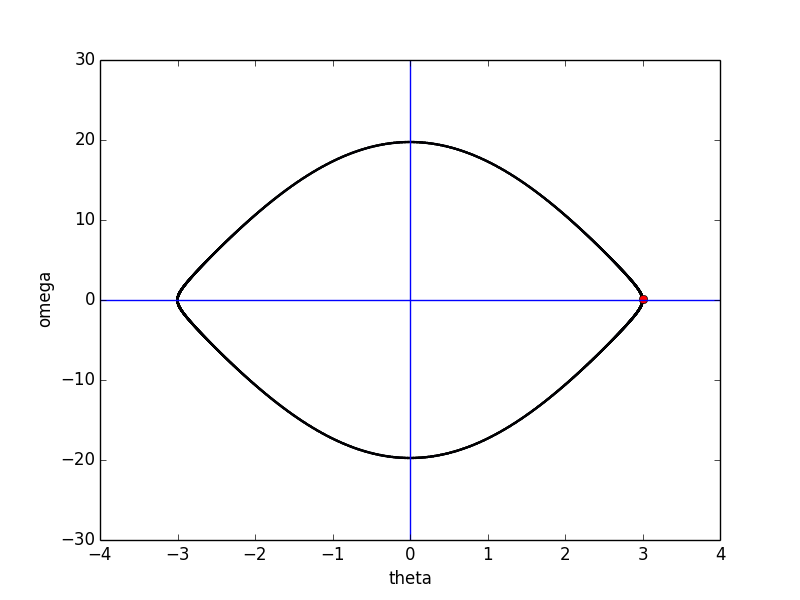
\includegraphics[height=2in]{figs/Q2_a.png}
  \caption{[$\theta$,$\omega$] = [3, 0.1]}
  \label{q2a}
\end{subfigure}%
\begin{subfigure}{.5\textwidth}
  \centering
  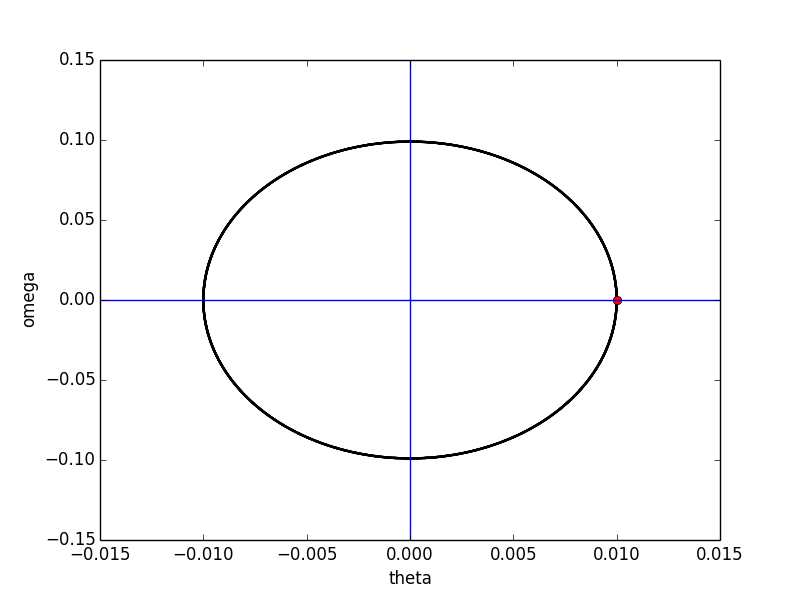
\includegraphics[height=2in]{figs/Q2_b.png}
  \caption{[$\theta$,$\omega$] = [0.01, 0]}
  \label{q2b}
\end{subfigure}
\caption{state-space trajectories}
\label{fig:test}
\end{figure}

Fig.\ref{q2a} shows the state-space trajectory starting from [$\theta$,$\omega$] = [3, 0.1] with $\Delta t = 0.005$. This initial condition is near an equilibrium point, namely [$\theta$,$\omega$] = [$\pi$, 0]. In order to see if that point is stable or unstable, we use a Jacobian matrix $A$ in order to linearly approximate vectors around that point as in \textit{Strogatz}. It turns out that  [$\theta$,$\omega$] = [$\pi$, 0] is a \textit{saddle point}, so it is unstable.

\subsubsection*{(b)}
Fig.\ref{q2b} shows the state-space trajectory with an initial condition [$\theta$,$\omega$] = [0.01, 0]. As one can see the shape of the orbit is more circular than the one in fig.\ref{q2a}.
As a trajectory gets closer to the saddle point, i.e., [$\theta$,$\omega$] = [$\pi$, 0], its form around the saddle point becomes more linear, thus looking less circular overall. Thus fig.\ref{q2b} looks "more" circular than its counterpart.

\begin{figure}
\centering
\begin{minipage}{.5\textwidth}
  \centering
  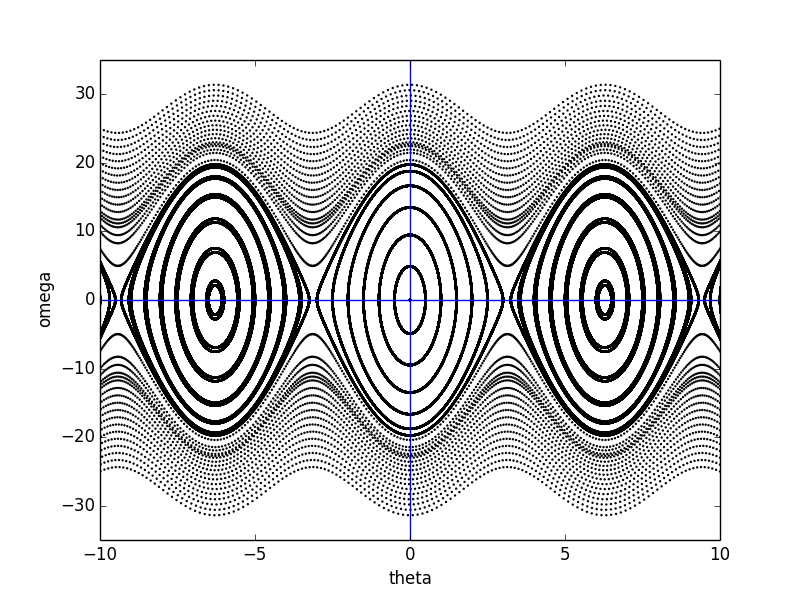
\includegraphics[height=2.5in]{figs/Q3.png}
  \captionof{figure}{state-space portrait of the pendulum}
  \label{q3}
\end{minipage}%
\begin{minipage}{.5\textwidth}
  \centering
  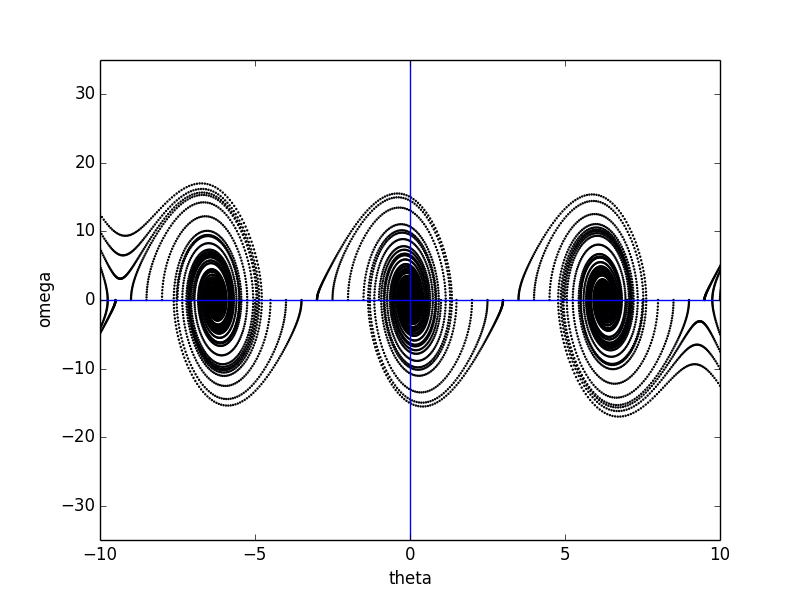
\includegraphics[height=2.5in]{figs/Q4.png}
  \captionof{figure}{state-space portrait of the pendulum with $\beta$ = 0.25}
  \label{q4}
\end{minipage}
\end{figure}

\subsection*{Problem 3}
Fig.\ref{q3} shows a state-space portrait of the pendulum.

\subsection*{Problem 4}
Fig.\ref{q4} shows the state-space portrait of the pendulum with $\beta$ = 0.25. what can be observed is that the closed orbits are not closed anymore and they are getting closer to the centers as time goes. Now the system is dissipative; the physical implication of this phenomenon is that the mass fixed to the pendulum loses its energy due to the friction $\beta$. If $\beta$ is large, the speed that the spiral gets to the center is faster and the opposite behavior appears for small $\beta$.

\subsection*{Problem 5}
Fig.\ref{q5} shows a state-space portrait of the pendulum for modulo $2\pi$. The modulo operation enables ones to show the overall behavior of the pendulum compactly.
\begin{figure}
  \centering
  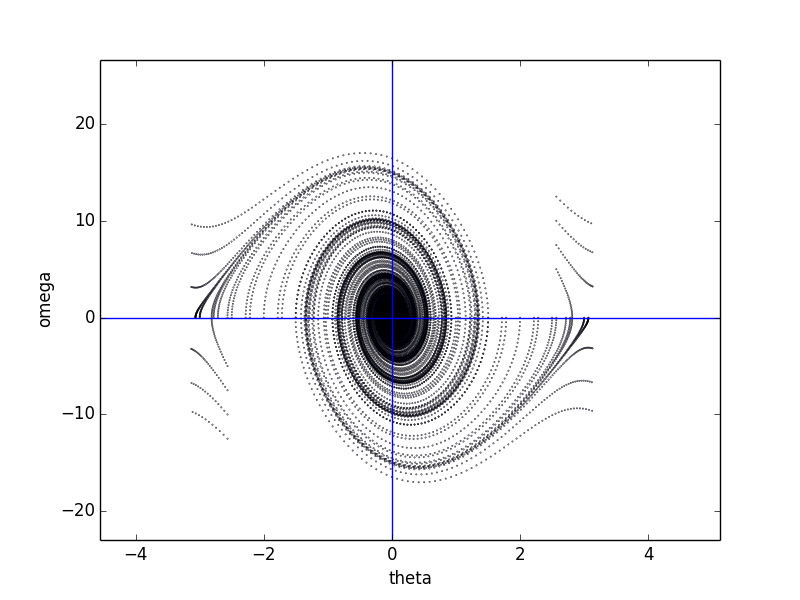
\includegraphics[height=3in]{figs/Q5_modified.png}
  \caption{state-space portrait of the pendulum for modulo $2\pi$}
  \label{q5}
\end{figure}

\subsection*{Problem 6}
Initially, we start with a value of the amplitude $A = 0.001$ and see a circle of the trajectory that does not diverge nor converge. Then if we increase the value, we observe  bifurcations of the trajectory, having multiple circles together centered at the origin. When we have $A = 1.05$, we observe the chaotic orbit, as shown in the fig.\ref{q6}.

\begin{figure}
  \centering
  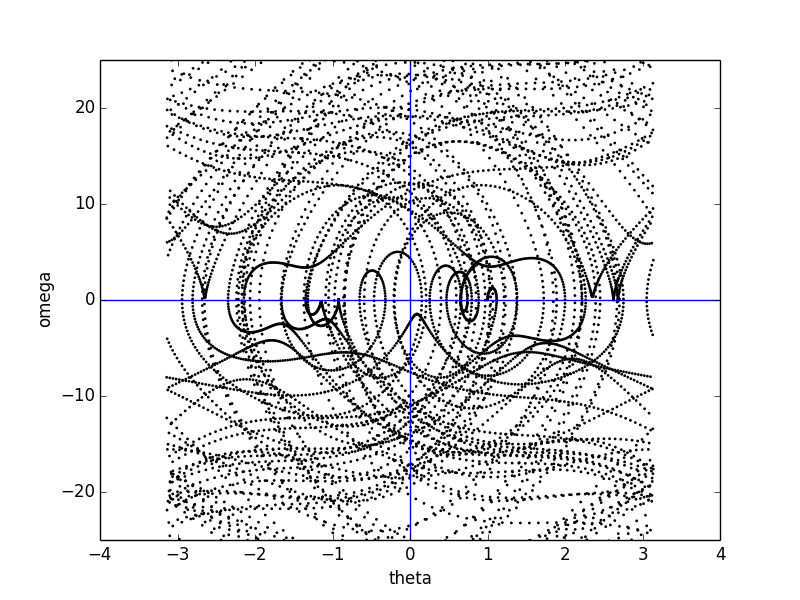
\includegraphics[height=3in]{figs/Q7/chaos_a105.png}
  \caption{state-space portrait of chaotic orbit. $\beta = 0.25$, $a=1.05$, $\alpha = \sqrt \frac{g}{l} \times \frac{3}{4}$}
  \label{q6}
\end{figure}

\subsection*{Problem 7}
Until a certain time step, increasing the value of $\Delta t$ makes the state-space trajectory converge to the origin [0, 0], this can be attributed to the fact that RK4 solver finds a next iteration point slightly inside the true trajectory. See figs \ref{q71} and \ref{q72}. Beyond a certain point (around $\Delta t = 0.5$), however, the trajectory diverges to the infinity. This is due to the RK4 solver's overshoot of finding the next iteration point.
\begin{figure}
\centering
\begin{subfigure}{.5\textwidth}
  \centering
  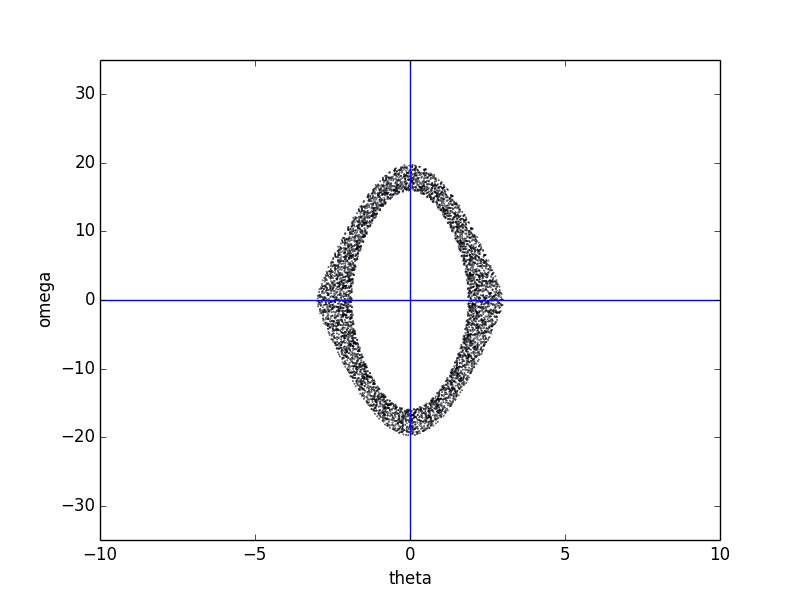
\includegraphics[height=2in]{figs/Q7/t005.png}
  \caption{$\Delta t = 0.05$}
  \label{q71}
\end{subfigure}%
\begin{subfigure}{.5\textwidth}
  \centering
  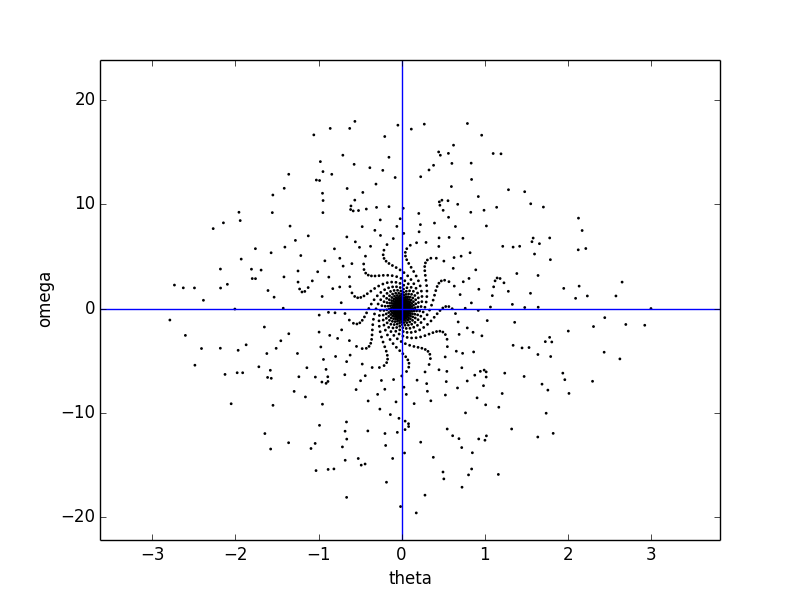
\includegraphics[height=2in]{figs/Q7/t01.png}
  \caption{$\Delta t = 0.1$}
  \label{q72}
\end{subfigure}
\caption{state-space trajectories with various $\Delta t$}
\label{fig:varying_t}
\end{figure}

\end{document}












